%%%%%%%%%%%%%%%%%%%%%%%%%%%%%%%%%%%%%%%%%%%%%%%%%%%%%%%%%%%%%%%%%%%%%%%%%%%%%%%%%%%%%
%%%%%%%%%%%%%%%%%%%%%%%%%%%%%%%%%%%%%%%%%%%%%%%%%%%%%%%%%%%%%%%%%%%%%%%%%%%%%%%%%%%%%
%%%%%%%%%%%%%%%%%%%%%%%%%%%%%%%%%%%%%%%%%%%%%%%%%%%%%%%%%%%%%%%%%%%%%%%%%%%%%%%%%%%%%
%%%%%%%%%%%%%%%%%%%%%%%%%%% STAN POCZATKOWY PROJEKTU %%%%%%%%%%%%%%%%%%%%%%%%%%%%%%%%
%%%%%%%%%%%%%%%%%%%%%%%%%%%%%%%%%%%%%%%%%%%%%%%%%%%%%%%%%%%%%%%%%%%%%%%%%%%%%%%%%%%%%
%%%%%%%%%%%%%%%%%%%%%%%%%%%%%%%%%%%%%%%%%%%%%%%%%%%%%%%%%%%%%%%%%%%%%%%%%%%%%%%%%%%%%
%%%%%%%%%%%%%%%%%%%%%%%%%%%%%%%%%%%%%%%%%%%%%%%%%%%%%%%%%%%%%%%%%%%%%%%%%%%%%%%%%%%%%

\chapter{Stan początkowy projektu}
\label{cha:pocz}

Niniejszy rozdział został przygotowany w oparciu o wiedzę przekazaną przez opiekuna pracy dr. hab. inż. Bartosza Mindura, pracę magisterskią mgr. Przemysława Pluteckiego pt. \textit{Aktualizacja oprogramowania oraz sprzetu elektronicznego dla Systemu Stabilizacji Wzmocnienia Gazowego TUTAJ DODAC REF MOZNA?} oraz pracę magisterską mgr. Pawła Zadrożniaka pt. \textit{Aktualizacja sprzętu elektronicznego dla Systemu Stabilizacji Wzmocnienia Gazowego TUTAJ DODAC REF MOZNA?}.

\section{Architektura}

Główna logika projektu została wykonana z użyciem języka C++, dzięki czemu aplikacja jest szybka i wydajna. Część kodu źródłowego została napisana z użyciem standardu 11. Wykorzystano również zewnętrzne biblioteki takie jak biblioteka Boost, czy też GSL. Początkowa architektura projektu oparta była o płaską strukturę folderów. Konwencja jaka została przyjęta, to \textbf{nazwaLib} dla folderów zawierających pliki bibliotek oraz \textbf{\_nazwa} dla folderów zawierających aplikacje uzytkowe.\par
\bigskip
Biblioteki, które były zawarte w ramach projektu, to:
\begin{itemize}
\item ggssLib - biblioteka zawierająca logikę aplikacji \textbf{ggssrunner}, czyli głownego programu wykonywalnego projektu
\item fifoLib - biblioteka implementująca kolejkę FIFO (first in first out)
\item FitLib - biblioteka wspierająca obliczenia numeryczne z wykorzystanie biblioteki zewnętrznej \textbf{GSL}
\item utilsLib - biblioteka zawierająca pliki pomocnicze projektu
\item xmlLib - biblioteka wykonywująca parsowanie pliku konfiguracyjnego aplikacji, który jest napisany w formacie \textbf{xml}
\item handleLib - biblioteka realizująca obsługuę mechanizmu sygnałów i slotów
\item logLib - biblioteka odpowiedzialna za mechanizm logowania
\item ThreadLib - biblioteka odpowiadająca za wykorzystanie wielowątkowości w aplikacji
\item CaenHVLib - biblioteka okalająca (ang. wrapper) bibliotekę \textbf{CaenN1470Lib}
\item CaenN1470Lib - biblioteka implementująca komunikację z urządzeniem sprzętowym \textbf{(CAEN N1470)}
\item OrtecMcbLib - biblioteka okalająca (ang. wrapper) bibliotekę \textbf{mcaLib}
\item mcaLib - biblioteka odpowiedzialna za komunikację z urządzeniem sprzętowym \textbf{(CAEN N957)}
\item usbrmLib - biblioteka, której zadaniem jest komunikacja z multiplekserami
\end{itemize}

\par Aplikacje, które były zawarte w ramach projektu, to:
\begin{itemize}
\item \_ggss - aplikacja ggssrunner, która odpowiada za człon projektu, jest to główny program wykonywalny
\item \_dimCS - aplikacja odpowiedzialna za wysyłanie komend, za pomocą technologii dim
\item \_ggssspector - aplikacja, której zadaniem zapisywanie parametrów pracy, np.: ustawione napięcie, odczytane napięcie, ciśnienie itp
\end{itemize}

\par Oprócz opisanych wcześniej katalogów występowały również:
\begin{itemize}
\item zawierające pliki nagłówkowe wspólne dla wielu bibliotek (include)
\item zawierakące biblioteki zewnętrzne (lib)
\item zawierające konfigurację aplikacji oraz skrypt pomocniczy w języku Python dla biblioteki serial (misc)
\item zawierające skrypty pomocnicze w języku Python i Bash oraz skrypty watchdog (obserwatorzy)
\end{itemize}

\par Dodatkowo projekt wykorzystywał następujące biblioteki zewnętrzne:
\begin{itemize}
\item Boost - biblioteka C++ ogólnego przeznaczenia
\item GSL (GNU Scietific Library) - biblioteka numeryczna dla języka C oraz C++
\item dim - biblioteka wspierająca komunikacja protokołem dim
\item QT oraz QWT - biblioteki wykorzystywane w ramach modułu GGSS Spector
\end{itemize}

W ramach projektu został również przygotowany panel informacyjno-administracyjny w technologii Scada (WinCC OA), który komunikuje się z główną cześcią aplikacji za pomocą protokołu dim. Rysunek \ref{fig:highLevelArch} przedstawia wysokopoziomową architekturę wraz z przepływem informacji.

\begin{figure}[H]
\centering
\caption{Wysokopoziomowa architektura projektu GGSS}
\label{fig:highLevelArch}
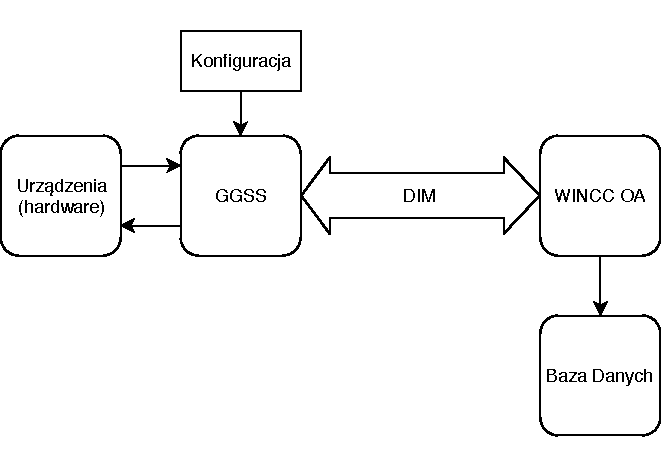
\includegraphics[width=\textwidth]{res/highLevelArch}
\end{figure}

W ramach architektury projektu utworzone zostały również pliki CMAKE, które służyły jako szablon akcji wykorzystywanych wielokrotnie w pozostałych miejscach, np.: wyszukiwanie odpowiedniej biblioteki.\par 
Architektura projektu charakteryzowała się całkowiecie płaską strukturą, nie było żadnej gradacji bibliotek, z której nie wynikały żadne zależności między modułami. Plusem takiego rozwiązania była łatwość w budowie całego systemu (np. brak problemów z skomplikowanymi ściezkami), aczkolwiek nie wynikała z niego żadna informacja nt. systemu ze względu na co próg wejścia, czy też utrzymanie projektu jest utrudnione. Widoczny był podział na moduły, lecz nie był on w żaden sposób uporządkowany, np. ze względu na przeznaczenie bibliotek (programowe, sprzętowe). 

\par Projekt zawierał również moduł przeznaczony obsłudze sterownika projektu ggss (ggss-driver). Zawierał on archiwum z sterownikiem dla urządzenia firmy Caen (CAEN N957) dostarczanym przez ww. firmę. W ramach modułu został również zawarty plik CMAKE, którego zadaniem było przygotowanie pakietu RPM w skład którego wchodził sterownik, biblioteki od firmy Caen (libCAENN957) oraz pre-generowane skrypty pozwalające na instalację oraz dezinstalację pakietu.

\section{Budowanie} 
Niniejsza część pracy zawiera opis pierwotnego sposobu budowania aplikacji, wraz z zastosowanymi rozwiązaniami technologicznymi (struktura i zawartość plików CMake) oraz listą potencjalnych ograniczeń wynikających z dotychczasowego podejścia do budowania.

\paragraph*{Struktura plików CMake}\mbox{}\\
% Opisac co gdzie jest, za co odpowiadają poszczegolne szablony
Projekt w swojej oryginalnej postaci budowany był za pomocą narzędzia CMake w wersji \textbf{2.8}. Wyróżnić można było jeden nadrzędny plik \textit{CMakeLists.txt} znajdujący się w katalogu głownym projektu oraz pomniejsze pliki dla każdego z modułów. Rysunek przedstawia w uproszczeniu pierwotną strukturę projektu, z wyszczególnieniem plików odpowiedzialnych za jego budowanie.

\textbf{TODO: tutaj dac jakis fajny rysuneczek}












\paragraph*{Obsługa bibliotek zewnętrznych}\mbox{}\\
% Opisac, jak obsługiwany jest Boost, GSL, Caen



\paragraph*{Ograniczenia pierwotnego systemu budowania}\mbox{}\\
% Cos jeszcze dopisac, zrobic zeby sie to lepiej czytalo
Pierwotna wersja projektu narzuca daleko idące ograniczenia na sposób jego budowania. Najważniejszym z nich jest brak bezpośredniej możliwości zbudowania pojedynczych komponentów projektu. Listing \ref{lst:orig} przedstawia fragment oryginalnego pliku \textit{CMakeLists.txt} znajdującego się w katalogu głównym projektu. \textbf{TUTAJ REF DO PRACY PLUTECKIEGO} Plik ten pozwala na zbudowanie trzech aplikacji wchodzących w skład oprogramowania projektu GGSS: \textit{ggssrunner}, \textit{dimCS} oraz opcjonalnie \textit{ggsspector}. Jest to jedyny plik w całym projekcie zawierający wszystkie informacje konieczne do zbudowania wymienionych aplikacji - tzn. posiadający listę bibliotek, od których aplikacje te są zależne. Oznacza to, że niemożliwe jest zbudowanie aplikacji \textit{ggssrunner} jedynie za pomocą dedykowanego jej pliku \textit{CMakeLists.txt}. Zatem pomimo, iż struktura projektu jest zmodularyzowana jeśli chodzi o architekturę (oprogramowanie zostało podzielone na biblioteki), to niemożliwe jest (w prosty sposób, za pomocą dostarczonych plików \textit{CMakeLists.txt}) zbudowanie pojedynczych modułów projektu.

\begin{lstlisting}[language=bash, caption={Fragment oryginalnego pliku CMakeLists.txt znajdującego się w katalogu głównym pierwotnej wersji projektu}, label={lst:orig}]
# array with used libraries
set(PROJECTS
        logLib
        xmlLib
        utilsLib
        handleLib
        ThreadLib
        fifoLib
        FitLib
        OrtecMcbLib
        CaenHVLib
        ggssLib
        usbrmLib
        CaenN1470Lib
        mcaLib
        daemonLib
        )

foreach (singleproject ${PROJECTS})
        parse_directory(${singleproject})
endforeach(singleproject)

# executables
add_subdirectory (_ggss) # ggssrunner binary
add_subdirectory (_dimCS) #dimCS binary
if(BUILD_GGSSPECTOR)
    add_subdirectory (_ggsspector) #ggsspector binary
endif()
\end{lstlisting}

Budowanie projektu za pomocą pliku, którego fragment przedstawia listing \ref{lst:orig} opiera się na liście zależności przechowywanej w zmiennej \textit{PROJECTS}. Umożliwia to stosunkowo łatwe rozszerzanie projektu o nowe biblioteki - wystarczy dopisać nazwę katalogu z biblioteką do listy zależności. Wadą tego rozwiązania jest natomiast brak możliwości wywnioskowania zależności zachodzących w projekcie. Listing \ref{lst:origggss} przedstawia plik \textit{CMakeLists.txt} służący do budowania aplikacji \textit{ggssrunner}. Na podstawie tych dwóch plików można jedynie wywnioskować, że aplikacja \textit{ggssrunner} jest zależna od wszystkich bibliotek, których nazwy znaleźć można w zmiennej \textit{PROJECTS}. Nie ma natomiast możliwości identyfikacji zależności między samymi bibliotekami. Takie podejście utrudnia zrozumienie struktury projektu, co bezpośrednio prowadzi do problemów z jego rozwojem.

%% Dodac bardziej szczegolowy opis tego projektu
\begin{lstlisting}[language=bash, caption={Oryginalny plik CMakeLists.txt służacy budowania aplikacji ggssrunner.}, label={lst:origggss}]
project (_ggss)
add_executable (ggssrunner main)
target_link_libraries (ggssrunner ${PROJECTS})
install(TARGETS ggssrunner RUNTIME DESTINATION bin)
\end{lstlisting}




\section{Dostarczanie i uruchamianie}

\section{Kontrola wersji}


%%%%%%%%%%%%%%%%%%%%%%%%%%%%%%%%%%%%%%%%%%%%%%%%%%%%%%%%%%%%%%%%%%%%%%%%%%%%%%%%%%%%%
%%%%%%%%%%%%%%%%%%%%%%%%%%%%%%%%%%%%%%%%%%%%%%%%%%%%%%%%%%%%%%%%%%%%%%%%%%%%%%%%%%%%%
%%%%%%%%%%%%%%%%%%%%%%%%%%%%%%%%%%%%%%%%%%%%%%%%%%%%%%%%%%%%%%%%%%%%%%%%%%%%%%%%%%%%%
%%%%%%%%%%%%%%%%%%%%%%%%%%% STAN DOCELOWY PROJEKTU %%%%%%%%%%%%%%%%%%%%%%%%%%%%%%%%%%
%%%%%%%%%%%%%%%%%%%%%%%%%%%%%%%%%%%%%%%%%%%%%%%%%%%%%%%%%%%%%%%%%%%%%%%%%%%%%%%%%%%%%
%%%%%%%%%%%%%%%%%%%%%%%%%%%%%%%%%%%%%%%%%%%%%%%%%%%%%%%%%%%%%%%%%%%%%%%%%%%%%%%%%%%%%
%%%%%%%%%%%%%%%%%%%%%%%%%%%%%%%%%%%%%%%%%%%%%%%%%%%%%%%%%%%%%%%%%%%%%%%%%%%%%%%%%%%%%

\chapter{Stan docelowy projektu}
\label{cha:docel}
Niniejszy rozdział zawiera opis docelowej wersji systemu GGSS, jaka powinna zostać osiągnięta po zakończeniu przez autorów prac. Cele do zrealizowania podzielone zostały na dwie główne części, wynikające z organizacji czasowej prac tzn. wkład autorów w system nie zamyka się wraz z zakończeniem prac nad niniejszym manuskryptem. Z tego powodu niniejszy rodział podzielony został na dwie części - pierwsza z nich opisuje finalną wersję projektu, natomiast druga - wersję po zakończeniu prac w ramach projektu inżynierkiego.

\section{Finalna wersja projektu}
Projekt w swojej wersji finalnej ma charakteryzować się modularną architekturą zarówno jeśli chodzi o organizację kodu, jak i sposób jego budowania. Pozwala to na proste i efektywne testowanie każdego komponentu z osobna. Ułatwia to również podmianę komponentów w środowisku produkcyjnym. Większa modularyzacja pozwala skrócić czas poszukiwania źródła ewentualnych błędów w działaniu systemu. Z drugiej natomiast strony podział systemu na dużą liczbę komponentów utrudnia proces budowania, przez co wymagana jest jego znacząca automatyzacja. Konieczne jest przygotowanie więc prostej w użytkowaniu infrastruktury wspomagającej proces produkcyjny. Powinna być ona dobrze udokumentowana, by próg wejścia do projektu był możliwie niski. Powinny więc zostać przygotowane instrukcje w języku angielskim zawierające zestaw najczęściej używanych komend wraz z wariantami ich użycia (np. flagi). Kluczowym celem jest również modernizacja kodu źródłowego - zarówno jeśli chodzi o jego jakość, jak i zastosowane technologie. Projekt charakteryzować się ma więc ustandaryzowanym, ogólnoprzyjętym przez społeczność programistów jako tzw. \textit{dobre praktyki}, nazewnictwem, odpowiednim podziałem na poziomie kodu źródłowego (funkcje, klasy itp.). W swojej ostatecznej wersji projekt powinien bazować na najnowszych, dostępnych w ramach infrastruktury produkcyjnej CERN-u, technologiach, np. standard języka C++. Dzięki temu zależności zewnętrzne powinny zostać ograniczone do minimum, na rzecz standardowych rozwiązań (np. biblioteka standardowa), by zagwarantować możliwie duża przenośność. Zaplanowano również rozszerzenie projektu o nowe komponenty ułatwiające korzystanie z systemu (np. graficzny interfejs użytkownika).

\section{Stan oczekiwany w ramach projektu inżynierskiego}
Z uwagi na brak możliwości realizowania wszystkich powyższych postulatów dotyczących celów pracy w ramach projektu inżynierkiego (co wynika z ograniczonego czasu), wybrany został następujący podzbiór wymagań:
\begin{itemize}
\item przygotowanie środowiska umożliwijącego zarządzanie prowadzonym projektem
\item modularyzacja projektu (z poziomu architektury i systemu budowania \textit{CMake})
\item przygotowanie infrastruktury automatyzującej proces produkcyjny, zapewniającej spójne środowisko do testowania
\item wykonanie dokumentacji zgodnej z wymienionymi założeniami
\item wprowadzenie standardu nazewnictwa na poziomie procesu budowania i podziału na repozytoria
\item przeprowadzenie testów wynikowego produktu
\end{itemize}
Rezultatem zakończenia tej części prac powinien być w pełni działający, udoskonalony system.


%%%%%%%%%%%%%%%%%%%%%%%%%%%%%%%%%%%%%%%%%%%%%%%%%%%%%%%%%%%%%%%%%%%%%%%%%%%%%%%%%%%%%
%%%%%%%%%%%%%%%%%%%%%%%%%%%%%%%%%%%%%%%%%%%%%%%%%%%%%%%%%%%%%%%%%%%%%%%%%%%%%%%%%%%%%
%%%%%%%%%%%%%%%%%%%%%%%%%%%%%%%%%%%%%%%%%%%%%%%%%%%%%%%%%%%%%%%%%%%%%%%%%%%%%%%%%%%%%
%%%%%%%%%%%%%%%%%%%%%%%%%%% OGRANICZENIA INFRASTRUKTURY %%%%%%%%%%%%%%%%%%%%%%%%%%%%%
%%%%%%%%%%%%%%%%%%%%%%%%%%%%%%%%%%%%%%%%%%%%%%%%%%%%%%%%%%%%%%%%%%%%%%%%%%%%%%%%%%%%%
%%%%%%%%%%%%%%%%%%%%%%%%%%%%%%%%%%%%%%%%%%%%%%%%%%%%%%%%%%%%%%%%%%%%%%%%%%%%%%%%%%%%%
%%%%%%%%%%%%%%%%%%%%%%%%%%%%%%%%%%%%%%%%%%%%%%%%%%%%%%%%%%%%%%%%%%%%%%%%%%%%%%%%%%%%%

\chapter{Ograniczenia dostępnej infrastruktury}
\label{cha:ogra}
Z uwagi na silny związek oprogramowania GGSS z infrastrukturą CERN oraz wymóg zapewnienia możliwości budowania projektu na należących do niej maszynach, przed autorami postawiony został szereg ograniczeń związanych z możliwymi do użycia technologiami oraz sposobem wykonywania pewnych operacji. Niniejszy rozdział stanowi opis najważniejszych z tych ograniczeń z uwzględnieniem ich wpływu na obraną przez autorów pracy ścieżkę rozwoju projektu.


\section{Ograniczone uprawnienia w środowisku docelowym}


\section{Wersje kompilatorów i interpreterów}
Dostępne wersje kompilatorów i interpreterów stanowią jeden z kluczowych czynników, który należy uwzględnić podczas wprowadzania zmian w istniejącym systemie, ponieważ definiują one możliwy do wykorzystania podzbiór technologii. W kontekście systemu GGSS ograniczenia te dotyczą przede wszystkim kompilatora języka C++ oraz interpretera języka Python. 

\paragraph*{Wersja kompilatora języka C++}\mbox{}\\
Dostępna w ramach infrastruktury projektu wersja kompilatora języka C++ to \textbf{g++ (GCC) 4.8.5}. Wspiera ona w pełni standard C++11, czyli funkcjonalności takie, jak referencje do r-wartości, wyrażenia lambda czy zakresowa pętla for \cite{GCC48}. Wersja ta nie wspiera niestety nowszych wydań języka (C++14/17).

\paragraph*{Wersja interpretera języka Python}\mbox{}\\
Domyślną wersją Pythona jest \textbf{Python 2.7.5}, jednak dostępny jest również Python 3 (w wersji \textbf{Python 3.6.8}). Z uwagi na wspomniany wcześniej koniec oficjalnego wsparcia dla Pythona 2, który ma nadejść wraz z początkiem 2020 roku, naturalnym jest więc wybór wersji 3. Infrastruktura projektu posiada jednak znaczące braki jeśli chodzi o dostępne dla wersji 3 biblioteki zewnętrzne - domyślnie nie jest np. dostępna biblioteka \textit{Beautiful Soup}, slużąca do przetwarzania dokumentów w formacie HTML. Niektóre popularne bibliteki i frameworki (np. \textit{PyTest} - wykorzystywany do przeprowadzania testów oprogramowania) nie są dostępne dla obu wersji Pythona. Taka sytuacja wymusza więc wykorzystanie narzędzia \textit{virtualenv} w celu ich instalacji w odizolowanym środowisku, nie mającym wpływu na infrastrukturę CERN-u.

\section{Wersja narzędzia budującego CMake}
Dostępna wersja narzędzia CMake stanowiła zdaniem autorów największe ograniczenie w czasie prac nad projektem. Na maszynach docelowych dostępna jest jedynie stara wersja \textbf{2.8.12.2}. Nowsza wersja (\textbf{3.14.6}) dostępna jest na niektórych z komputerów, jednak z uwagi na konieczność zachowania kompatybilności ze wspomnianymi maszynami docelowymi, nie było możliwe jej użycie. Stosowanie wersji o numerze niższym od \textbf{3.0} skutkuje szeregiem ograniczeń - brakuje w niej wielu funkcjonalności pozwalających na stosowanie ogólnoprzyjętych dziś praktyk, jak np. określenie zakresu wersji narzedzia CMake, w którym powinna mieścić się używana wersja, by projekt można było bez problemu zbudować, czy wsparcie dla instrukcji \textit{target\_link\_directories} \cite{NewInCMake}.

\section{Związek projektu z wersją jądra systemu}


%%%%%%%%%%%%%%%%%%%%%%%%%%%%%%%%%%%%%%%%%%%%%%%%%%%%%%%%%%%%%%%%%%%%%%%%%%%%%%%%%%%%%
%%%%%%%%%%%%%%%%%%%%%%%%%%%%%%%%%%%%%%%%%%%%%%%%%%%%%%%%%%%%%%%%%%%%%%%%%%%%%%%%%%%%%
%%%%%%%%%%%%%%%%%%%%%%%%%%%%%%%%%%%%%%%%%%%%%%%%%%%%%%%%%%%%%%%%%%%%%%%%%%%%%%%%%%%%%
%%%%%%%%%%%%%%%%%%%%%%%%%%% WYKONANE PRACE %%%%%%%%%%%%%%%%%%%%%%%%%%%%%%%%%%%%%%%%%%
%%%%%%%%%%%%%%%%%%%%%%%%%%%%%%%%%%%%%%%%%%%%%%%%%%%%%%%%%%%%%%%%%%%%%%%%%%%%%%%%%%%%%
%%%%%%%%%%%%%%%%%%%%%%%%%%%%%%%%%%%%%%%%%%%%%%%%%%%%%%%%%%%%%%%%%%%%%%%%%%%%%%%%%%%%%
%%%%%%%%%%%%%%%%%%%%%%%%%%%%%%%%%%%%%%%%%%%%%%%%%%%%%%%%%%%%%%%%%%%%%%%%%%%%%%%%%%%%%

\chapter{Wykonane prace}
\label{cha:prace}

\section{Wykorzystanie funkcjonalności portalu Gitlab wspierających zarządzanie projektem}

\section{Migracja projektu do systemu kontroli wersji Git i zmiany w architekturze}

\section{Zastosowanie podejścia CI/CD}
% Czym jest CI/CD
% Realiacja za pomocą platformy gitLab
%   - mozliwe opcje, czemu nie autodevops
%   - pipeline (z przykladem)
%   - artefakty i ich znaczenie w GGSS
%   - pliki .yml (z przykladem)

\section{Zmiana sposobu budowania aplikacji}
% Zarys rozwiazania
% Szablony + Boost + GSL
% Budowanie bibliotek
% Budowanie aplikacji
% DIM - skrypt do pobierania, budowanie jak external_project
% Skrypty do budowania calosci (+ sposoby budowania) + glowny CMake

\section{Budowanie i dystrybucja sterownika oraz aplikacji testującej}

\section{Maszyna wirtualna oraz konteneryzacja - Docker}

\section{Pomniejsze prace}
\subsection{Integracja bibliotek napisanych w języku C z aplikacją w C++}
\subsection{Integracja zewnętrznej biblioteki dynamicznej z użyciem narzędzia CMake}

\section{Dokumentacja projektu}
% Czemu potrzebna
% Realizacja - pliki README.md, one-linery

